%
% LaTeX report template 
%

% This is a comment: in LaTeX everything that in a line comes
% after a "%" symbol is treated as comment

\documentclass[11pt, a4paper]{article}
\usepackage{graphicx}
\usepackage{amsmath}
\usepackage{listings}


\title{Assignment No 3} % Title

%\author{M.V.A.Suhas kumar (EE17B109)} % Author name
\author{M.V.A.Suhas Kumar \\ {\small EE17B109}}

\date{\today} % Date for the report
\begin{document}		
		
\maketitle % Insert the title, author and date
\section{Fitting Data to Models}
%Create new section;it is autonumbered
This week’s Python assignment is mainly focused on studying the effect of noise on the fitting process.\\
Firstly,we generated a file fitting.dat with 10 columns with first column as time ,while the remaining columns are data\\
The data columns correspond to the function with different amounts of noise added.Here,noise random fluctuations in the value due to many small random effects.Noise is assumed to be normally distributed.\\

Each column function with given $\sigma$:\\
\begin{equation*}
f(t) = 1.05J_{2}(t) - 0.105t + n(t)
\end{equation*}

with \begin{equation*}
Pr(n(t)|\sigma) = \frac{1}{\sigma\sqrt{2\pi}}exp(\frac{-n(t)^2}{2\sigma^2})
\end{equation*}

\begin{figure}[!tbh]
   	\centering
   	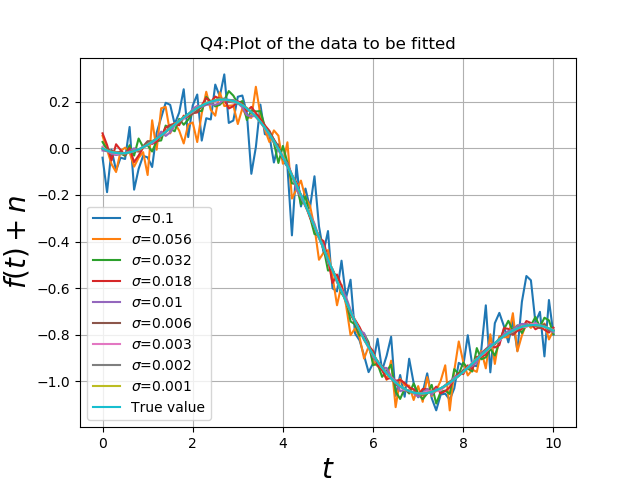
\includegraphics[scale=0.4]{q4_plot.png}  % Mention the image name within the curly braces. Image should be in the same folder as the tex file. 
   	\caption{Plot of data to be fitted}
   	\label{fig:Data plot}
   \end{figure} 
\newpage
Here I am plotting the error bar for one data column:\\
\begin{figure}[!tbh]
   	\centering
   	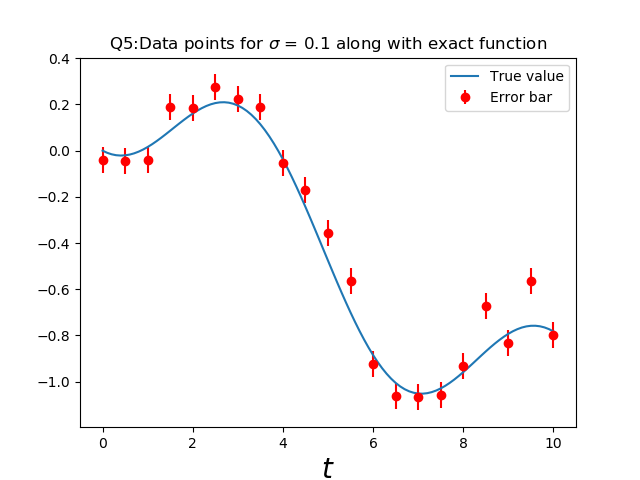
\includegraphics[scale=0.4]{q5_plot.png}  % Mention the image name within the curly braces. Image should be in the same folder as the tex file. 
   	\caption{Data points for $\sigma$ = 0.1 along with exact function}
   	\label{fig:Error bar}
   \end{figure}
   
True value function is plotted by defining a function:\\
\begin{equation*}
g(t,A,B) = AJ_{2}(t)+Bt 
\end{equation*}
Next we assume that there exist some function which fits the noise data  with general form  $g(t,A,B) = AJ_{2}(t)+Bt$\\
\par
Next we will find the (A,B) values by minimising the mean square error between the predicted values from given (A,B) and data column.\\

Contour Plot of $MS\ error$ for w.r.t data column1 for range of (A,B):
\begin{figure}[!tbh]
   	\centering
   	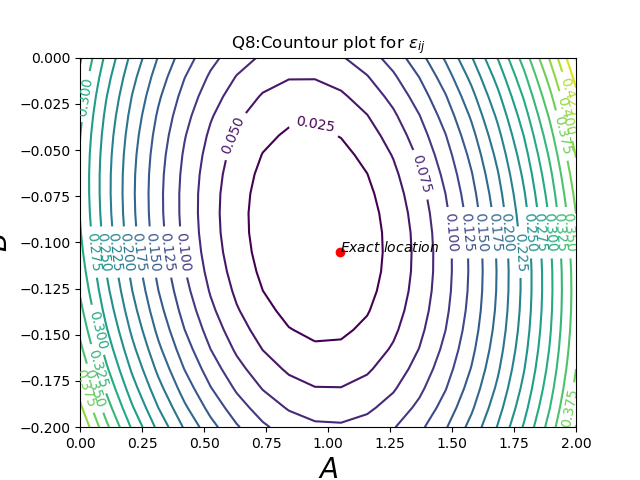
\includegraphics[scale=0.5]{q8_plot.png}  % Mention the image name within the curly braces. Image should be in the same folder as the tex file. 
   	\caption{contour plot for $\epsilon_{ij}$ }
   	\label{fig:Contour plot}
   \end{figure}

From the above plot we can clearly see that there exist a single minima.
\newpage
Using the Python function lstsq from scipy.linalg to obtain the best estimate of A and B for different data columns:\\

The following plots show the error in A and B for different data columns:\\

In the first plot B error is appearing to be constant but in reality it increases by a small amount.\\ 

\begin{figure}[!tbh]
   	\centering
   	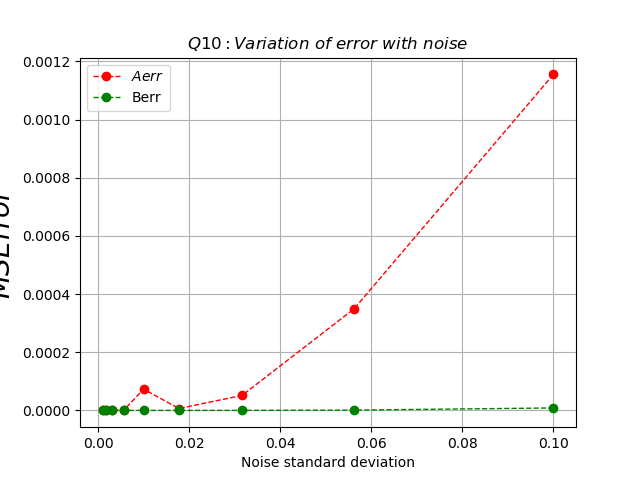
\includegraphics[scale=0.5]{q10_plot.png}  % Mention the image name within the curly braces. Image should be in the same folder as the tex file. 
   	\caption{A and B error in linear scale}
   	\label{fig:A and B err in linear scale}
   \end{figure}
\begin{figure}[!tbh]
   	\centering
   	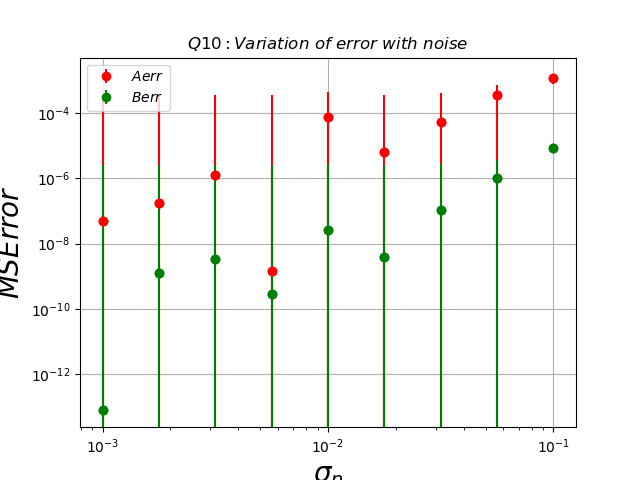
\includegraphics[scale=0.5]{q11_plot.png}  % Mention the image name within the curly braces. Image should be in the same folder as the tex file. 
   	\caption{A and B error in log scale}
   	\label{fig:A and B err in log scale}
   \end{figure}
\newpage

Here I am plotting mean square error of predicted points w.r.t to true points versus sigma of noise.

\begin{figure}[!tbh]
   	\centering
   	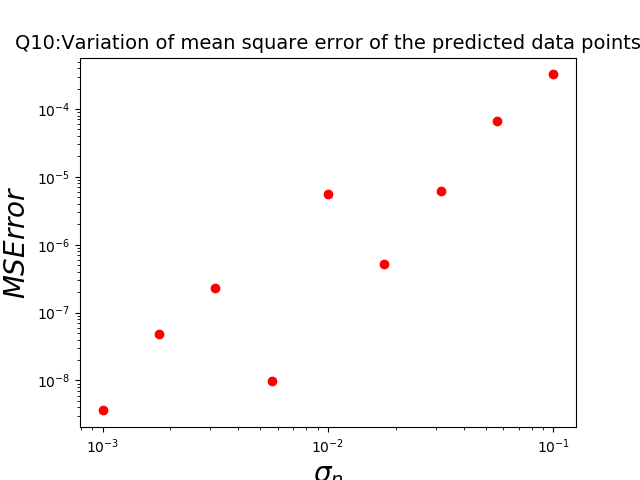
\includegraphics[scale=0.5]{Figure_1.png}  % Mention the image name within the curly braces. Image should be in the same folder as the tex file. 
   	\caption{Mean square error for predicted points}
   	\label{fig:pred mean square}
   \end{figure}
   
\textbf{Conclusion:}
If we calculate the mean square error for the predicted points w.r.t to the data points,In the log scale we observe that there will be a linear variation.


 
\end{document}



 
